This section shows the experimental and expected results of controlling a single joint via the Hubo-Ach system.
In this example the right shoulder pitch (RSP) is given a step input from 0.0 $rad$ to 0.4 $rad$.
The reference position $\theta_r$ is begin recorded as well as the actuator setpoint $\theta_c$ and the actual position of the joint $\theta_a$.
These definitions are also available in Table~\ref{table:recorded}

\begin{table}
\centering
\caption{States being recorded for the single joint step response test}
\begin{tabular}{l || c | c | c | c}
Signal      & Symbol     & Definition                    & Source      & Units \\
\hline
\hline
FeedForward & $\theta_r$ & Desired reference on the      & Hubo-Ach   & $rad$ \\
            &            & Hubo-Ach FeedForward Channel  &            &       \\
\hline
FeedForward & $\theta_c$ & Reference set to the actuator & Hubo-Ach   & $rad$ \\
\hline
Feedback    & $\theta_a$ & Actual position of joint as   & JMC        & $rad$ \\
            &            & measured from the encoders    &            &       \\
\hline
\end{tabular}
\label{table:recorded}
\end{table}



\begin{figure}[thpb]
  \centering
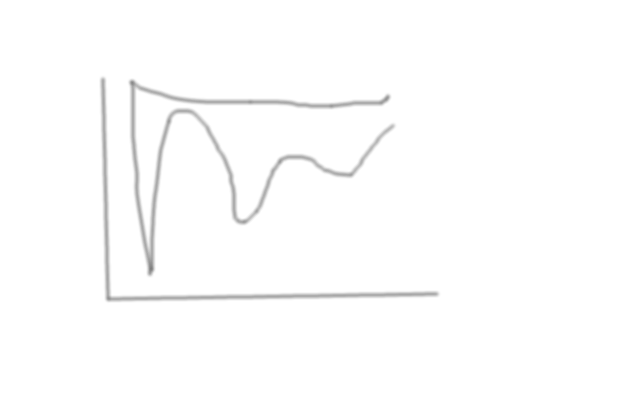
\includegraphics[width=0.8\columnwidth]{./pix/tmp.png}
  \caption{The commanded reference plotted against the actual reference recorded via Hubo-Ach and ground truth via CAN analyzing utilities.  In this plot the commanded reference is not automatically filtered by Hubo-Ach.  The commanded joint is the right shoulder pitch.}
  \label{fig:singleJointStep}
\end{figure}

Fig.~\ref{fig:singleJointStep} shows the results when a step input is applied and Hubo-Ach is in \textit{HUBO\_REF\_MODE\_REF\_FILTER} also know as pass-through mode.
This sets the what the desired reference on the \textbf{FeedForward} Hubo-Ach channel to the actuator's reference, i.e.:

\begin{equation}\label{eq:refrefmode}
 \theta_c(N) = \theta_r(N)
\end{equation}

Fig.~\ref{fig:hubo-ach-feedforward} shows the block diagram of the control setup.

\begin{figure}
\centering
\begin{tikzpicture}[->,>=stealth',shorten >=1pt,auto,node distance=5cm,
  thick,main node/.style={fill=white!20,draw,font=\sffamily\Large\bfseries}]


  \node[main node] (ref) {Reference};
  \node[main node] (hubo-ach) [right of=ref] {Hubo-Ach};
  \node[main node] (hubo) [right of=hubo-ach] {Hubo};




  \path[<->,dashed, every node/.style={font=\sffamily\small}]
    (hubo) edge node [above] {CAN} (hubo-ach);

  \path[->,every node/.style={font=\sffamily\small}]
    (ref) edge node [above] {$\theta_r$} (hubo-ach);


\end{tikzpicture}
\caption{Reference $\theta_r$ being applied to Hubo via Hubo-Ach.  $\theta_r$ is set on the \textbf{FeedForward} channel, Hubo-Ach reads it then commands Hubo at the rising edge of the next cycle.}
\label{fig:hubo-ach-feedforward}
\end{figure}






As seen in Fig~\ref{fig:singleJointStep} $\theta_c$ tracks $\theta_r$ perfectly. As expected $\theta_a$ lags by a minimum of 1 time step $T$.  
This is the time it takes between sending $\theta_c$ to the actuator over the CAN bus plus the time it takes in receiving the feedback from the encoder of the motor over CAN.
The remainder of the lag is due to the rise time of the actuator.
This is different for each joint.
Because all major joints are high-gain PID the rise-time and overshoot is very small which makes the robot very stiff.
The total lag between commanding the joint on the \textbf{FeedForward} channel and the response of the actuator is:

\begin{equation}
t_{lag} = t_{filter} + t_{rise}
\end{equation}



